\documentclass{beamer}
%\documentclass[handout]{beamer}
\usetheme{Antibes}

\setbeamertemplate{bibliography item}{\insertbiblabel}

\usepackage[ngerman]{babel}
\usepackage[utf8]{inputenc}
\usepackage{url}


\title{Untersuchung der Auswirkungen von Quantisierung und Pruning auf Convolutional Neural Networks für Mobilgeräte}
\author{Julian Hoever}
\date{31. März 2021}


\begin{document}


%%% Titelblatt %%%

\begin{frame}
\titlepage
\end{frame}



%%% Inhaltsverzeichnis %%%

\begin{frame}
\frametitle{Inhaltsverzeichnis}

\tableofcontents
\end{frame}

%%% Abschnitt: Einleitung %%%

\section{Einleitung \& Motivation}
\begin{frame}
\frametitle{Einleitung}

\begin{itemize}
	\item Convolutional Neural Networks für die Bildverarbeitung
	\item Viele Architekturen sind zu groß um auf Mobilgeräten verwendet zu werden
	\item Optimierte Architekturen für mobile/eingebettete Systeme
	\begin{itemize}
		\item MobileNet, MobileNetV2, MobileNetV3 und EfficientNet
		\item Architekturelle Optimierungen
	\end{itemize}
	\item Optimierungstechniken: Quantisierung und Pruning
\end{itemize}

\end{frame}


\begin{frame}
\frametitle{Motivation}

\begin{itemize}
	\item Architekturen können unterschiedlich auf die Anwendung von Quantisierung und Pruning reagieren
	\item Gibt es Architekturen die sich besonders gut für solche Optimierungen eignen?
\end{itemize}

\end{frame}



%%% Abschnitt: Grundlagen %%%

\section{Grundlagen}
\begin{frame}
\huge
\centering
Grundlagen
\end{frame}


\begin{frame}
\frametitle{MobileNet (2017) \cite{howard_mobilenets_2017}}

\begin{itemize}
	\item Zielsetzung: Verwendung von CNN Modellen auf mobilen/eingebetteten Systemen (möglichst niedrige Latenz)
	\item Aufgebaut aus Depthwise Separable Convolutions
\end{itemize}

\begin{figure}
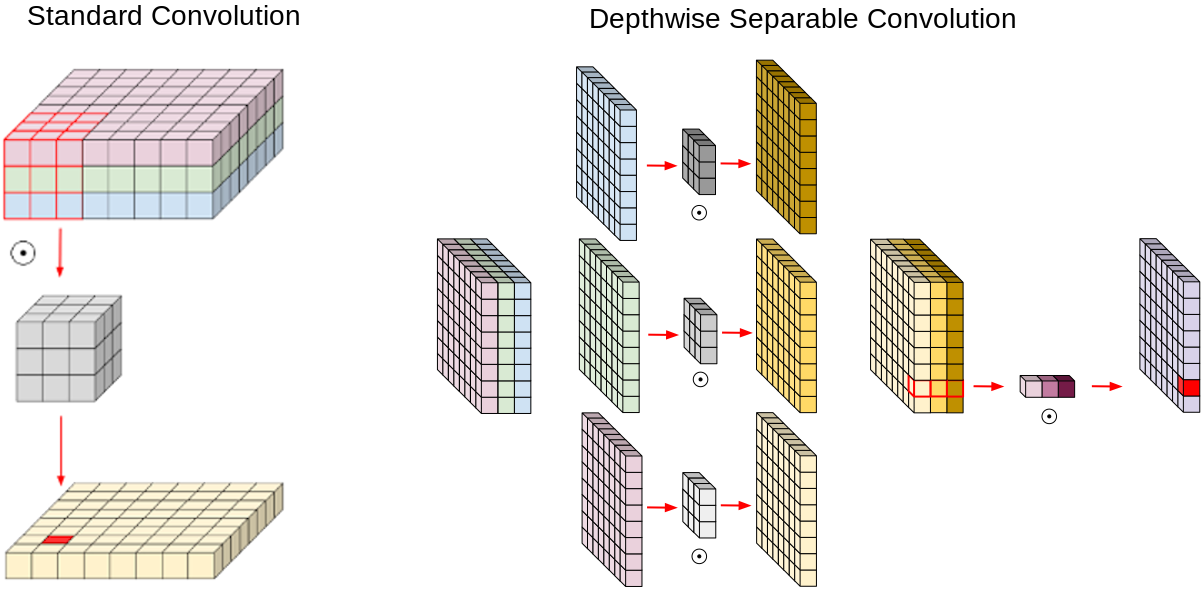
\includegraphics[width=0.7\textwidth]{img/depthwise_separable.png}
\caption{Schema einer Depthwise Separable Convolution \footnote{\url{https://eli.thegreenplace.net/2018/depthwise-separable-convolutions-for-machine-learning/}}}
\end{figure}

\end{frame}


\begin{frame}
\frametitle{MobileNetV2 (2018) \cite{sandler_mobilenetv2_2019}}

\begin{itemize}
	\item Nachfolger von MobileNet
	\item Verwendet ebenfalls Depthwise Separable Convolutions
	\item Neu hinzugekommen: Linear Bottlenecks und Inverted Residuals
	\item Hauptbaustein ist der Inverted Residual Block
\end{itemize}

\begin{figure}
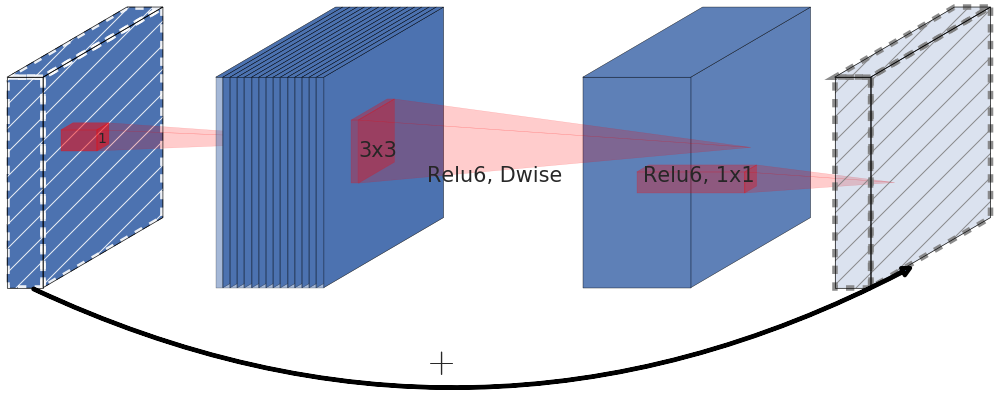
\includegraphics[width=0.6\textwidth]{img/inverted_residual.png}
\caption{Inverted Residual Block mit Linear Bottleneck \cite{sandler_mobilenetv2_2019}}
\end{figure}

\end{frame}


\begin{frame}
\frametitle{MobileNetV3 Large/Small (2019) \cite{howard_searching_2019}}

\begin{itemize}
	\item Mittels Platform-Aware Neural Architecture Search entwickelt
	\begin{itemize}
		\item Latenz wird auf Google Pixel Smartphones gemessen
		\item MobileNetV3 Large basiert auf der MnasNet-A1 Architektur
		\item Neuer Platform-Aware NAS Durchlauf für MobileNetV3 Small
	\end{itemize}
	\item NetAdapt Algorithmus und manuellen Anpassungen
	\item MobileNetV3 verwendet Squeeze-And-Excitation Module
\end{itemize}

\begin{figure}
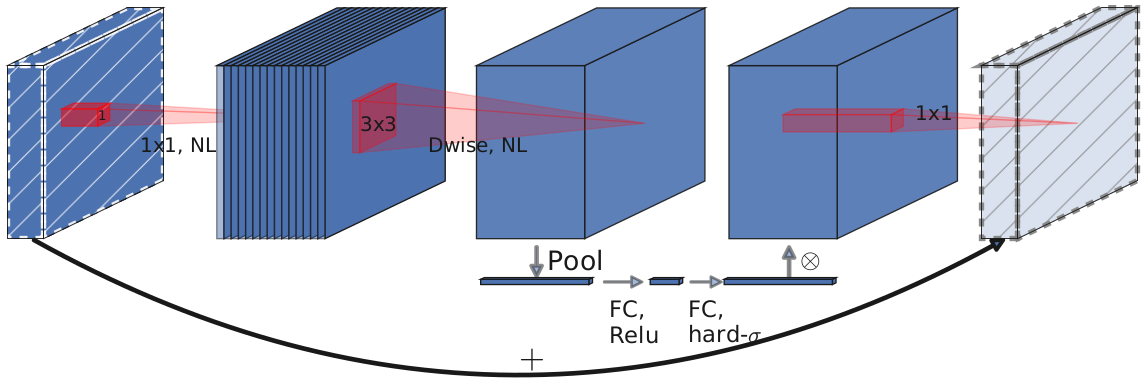
\includegraphics[width=0.8\textwidth]{img/mobilenetv3_block.png}
\caption{MobileNetV3 Building Block \cite{howard_searching_2019}}
\end{figure}

\end{frame}


\begin{frame}
\frametitle{EfficientNet (2019) \cite{tan_efficientnet_2020}}

\begin{itemize}
	\item Ziel: skalierbare Architektur um einen optimalen Trade-Off zwischen Genauigkeit und Ressourcenbedarf zu erreichen
	\item Mittels Neural Architecture Search entwickelt
	\begin{itemize}
		\item Nicht für eine spezielle Hardware optimiert
		\item Optimierung auf Gleitkommazahlen-Operationen
		\item Basisarchitektur EfficientNet-B0
	\end{itemize}
	\item Compound Scaling
	\item EfficientNet-B0 bis EfficientNet-B7
	\item Hauptbausteine ähneln dem MobileNetV3
\end{itemize}

\end{frame}


\begin{frame}
\frametitle{Quantisierung}

\begin{itemize}
	\item Darstellung eines Netzwerkes verkleinern
	\begin{itemize}
		\item Gewichte und Aktivierungen in eine Darstellung überführen, die weniger Bits benötigt.
	\end{itemize}
	\item Post-Training Quantisierung
	\begin{itemize}
		\item Bereits trainiertes Netzwerk wird ohne erneutes Training quantisiert.
	\end{itemize}
	\item Quantisierungsschema von TensorFlow \cite{jacob_quantization_2017}
	\begin{itemize}
		\item Reelle Zahl $r$ wird durch quantisierten Wert $q$ wie folgt dargestellt:
		\[r = S(q - Z)\]
		\item $S$, $Z$ sind Konstanten
	\end{itemize}
	\item In dieser Arbeit: Post-Training Float-Fallback Quantisierung
\end{itemize}

\end{frame}


\begin{frame}
\frametitle{Pruning}

\begin{itemize}
	\item Nicht benötigte Verbindungen werden gekappt
	\begin{itemize}
		\item Gewichte mit geringem Einfluss werden auf 0 gesetzt
	\end{itemize}
	\item Magnitude Pruning \cite{zhu_prune_2017}
	\begin{itemize}
		\item Anteil der auf 0 gesetzten Gewichte (Sparsity)
		\item Training und Pruning im Wechsel
		\item Schrittweise werden die kleinsten Gewichte einer Gewichtsmatrix auf 0 gesetzt. 
	\end{itemize}
\end{itemize}

\begin{figure}
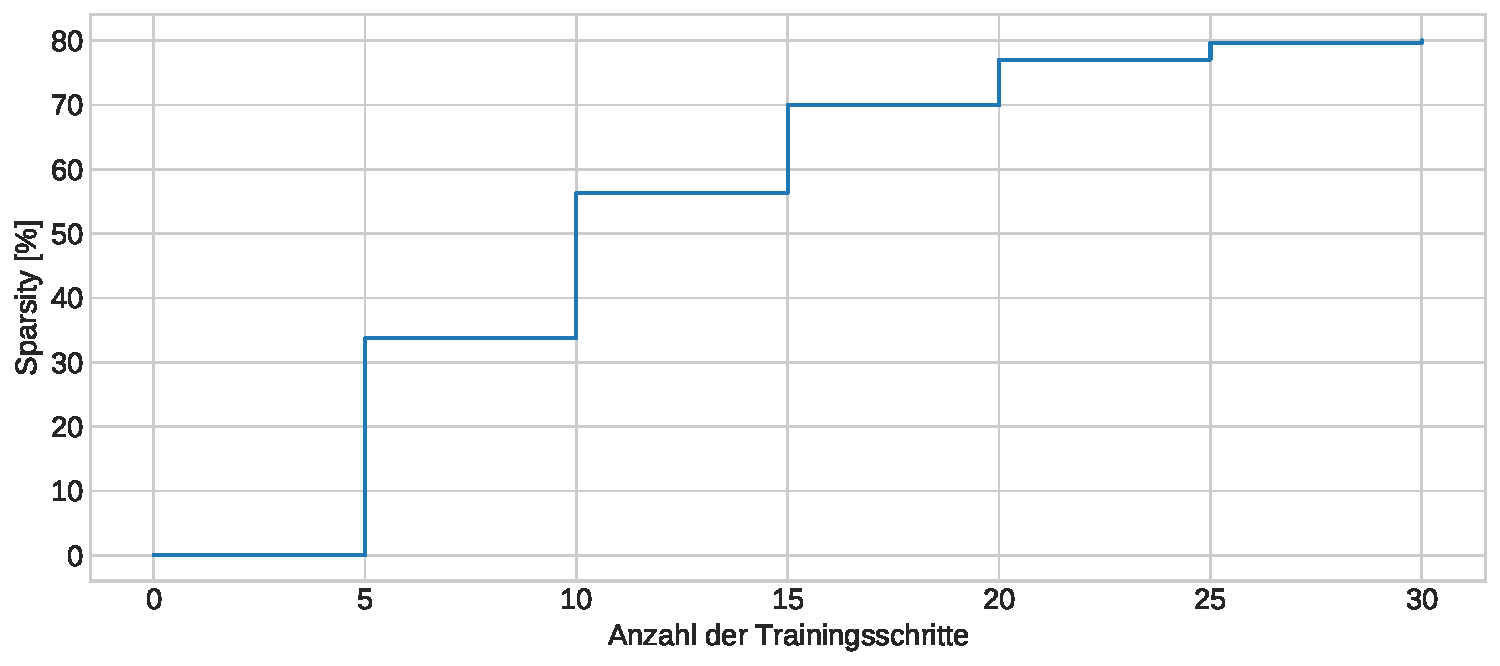
\includegraphics[width=0.6\textwidth]{img/magnitude_pruning_schedule.pdf}
\caption{Schrittweises Pruning}
\end{figure}

\end{frame}



%%% Abschnitt: Implementierung %%%

\section{Vorgehen}
\begin{frame}
\huge
\centering
Vorgehen
\end{frame}


\begin{frame}
\frametitle{Vorgehen}

\begin{itemize}
	\item Architekturen werden auf dem CIFAR-10 Datensatz trainiert
	\item Pruning und Quantisierung werden auf die Architekturen angewendet
	\item Folgende Kombinationen von Optimierungen werden untersucht:
	\begin{itemize}
		\item vortrainiert (keine Optimierungen)
		\item vortrainiert und quantisiert
		\item vortrainiert und gepruned
		\item vortrainiert, gepruned und quantisiert
	\end{itemize}
	\item TFLite FlatBuffer Format wird als einheitliches Format für die Speicherung der Modelle verwendet
	\item Modelle werden auf einem Raspberry Pi 4B ausgewertet
\end{itemize}

\end{frame}



%%% Abschnitt: Ergebnisse %%%

\section{Ergebnisse}
\begin{frame}
\huge
\centering
Ergebnisse
\end{frame}


\begin{frame}
\frametitle{Training}

\begin{itemize}
	\item Training mittels einheitlichem Setup
	\item Overfitting der Architekturen
	\item MobileNetV3 Architekturen ließen sich schwierig trainieren
	\item Hohe Inferenzzeit des EfficientNet-B0 im Gegensatz zum MobileNetV3 Large
\end{itemize}

\begin{table}
\tiny
\centering
\begin{tabular}{lllllll}
\hline
    Architekturen & Parameter & Top-1  & Top-3  & Datei [MB] & RAM [MB] & Inferenz [µs] \\
\hline
        MobileNet &  3.2 Mio. & 0.7277 & 0.9226 &    12.8453 &  16.1016 &         11803 \\
      MobileNetV2 &  2.3 Mio. & 0.7325 & 0.9263 &    8.9153 &  11.2148 &          4961 \\
MobileNetV3 Large &  4.2 Mio. & 0.6934 & 0.9064 &   16.8829 &  20.4141 &          8051 \\
MobileNetV3 Small &  1.5 Mio. & 0.6687 & 0.9033 &    6.1536 &   8.5859 &          2954 \\
  EfficientNet-B0 &  4.1 Mio. & 0.7514 & 0.9296 &   16.0860 &  16.6719 &         12453 \\
\hline
\end{tabular}
\caption{Zusammenfassung verschiedener Metriken nach dem Training}
\end{table}

\end{frame}


\begin{frame}
\frametitle{Quantisierung I}

\begin{itemize}
	\item Quantisierung verkleinert die Architekturen stark
	\item Geringe bis teilweise keine Verluste an Genauigkeit
	\begin{itemize}
		\item Ausnahme: MobileNetV3
	\end{itemize}	
	\item Inferenzzeit verringert sich stark (besonders bei der MobileNet Architektur)
\end{itemize}

\begin{table}
\tiny
\centering
\begin{tabular}{lllllll}
\hline
    Architekturen & Parameter &  Top-1 &  Top-3 &  Datei [MB] &  RAM [MB] &  Inferenz [µs] \\
\hline
        MobileNet &  3.2 Mio. & 0.7401 & 0.9312 &      3.6149 &   6.01560 &           3750 \\
      MobileNetV2 &  2.3 Mio. & 0.7507 & 0.9411 &      2.8626 &   6.91410 &           2843 \\
MobileNetV3 Large &  4.2 Mio. & 0.3963 & 0.7743 &      4.9440 &   6.93359 &           5259 \\
MobileNetV3 Small &  1.5 Mio. & 0.6349 & 0.8926 &      1.9539 &   5.20310 &           2183 \\
  EfficientNet-B0 &  4.1 Mio. & 0.7464 & 0.9324 &      5.1753 &   9.63670 &           8629 \\
\hline
\end{tabular}
\caption{Metriken nach Anwendung von Quantisierung}
\end{table}

\end{frame}


\begin{frame}
\frametitle{Quantisierung II}

\begin{figure}
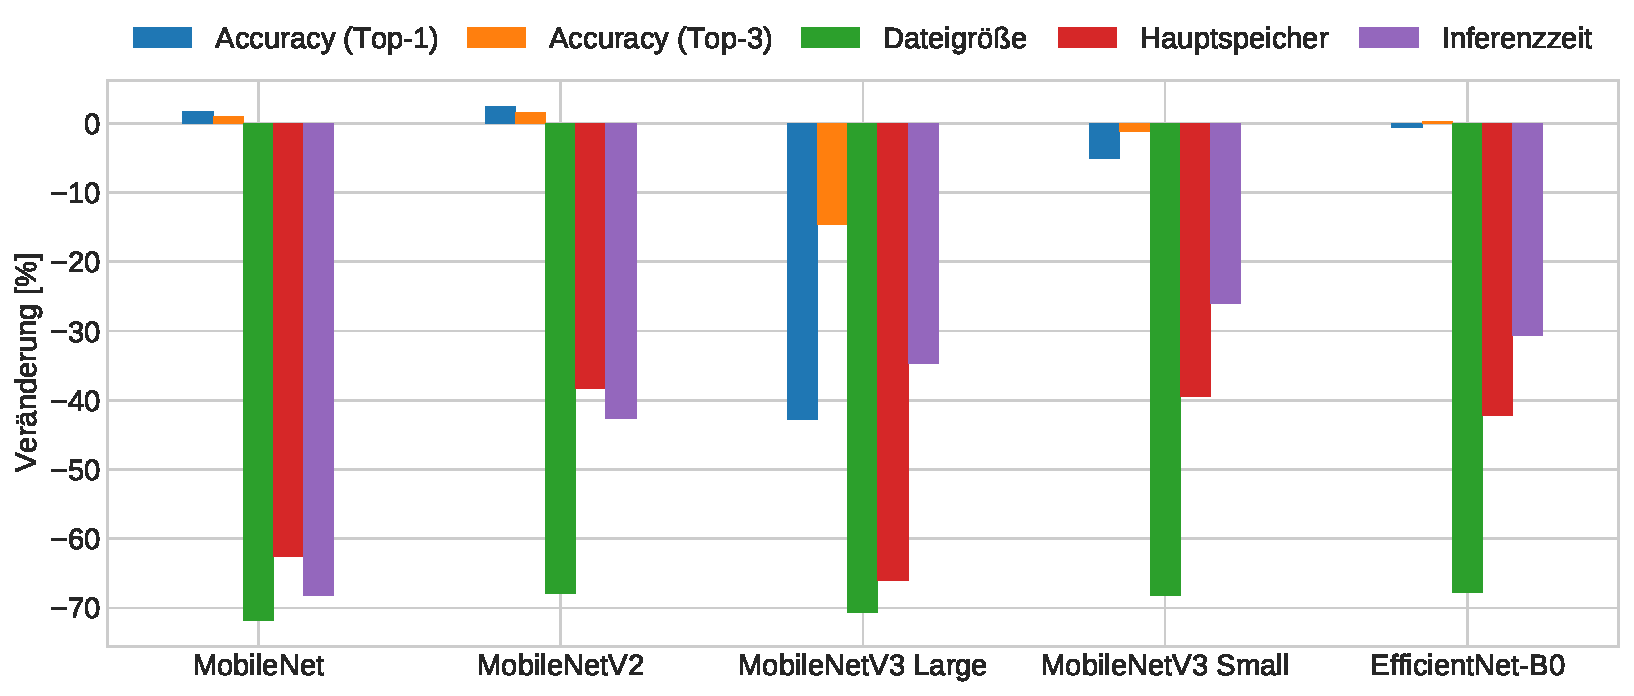
\includegraphics[width=0.9\textwidth]{img/quantization_improvements.pdf}
\caption{Veränderung der klassenweisen Top-1 Genauigkeit der geprunten MobileNet Modelle}
\end{figure}

\end{frame}


\begin{frame}
\frametitle{Pruning I}

\begin{itemize}
	\item Mit zunehmender Sparsity sinkt die Genauigkeit
	\item MobileNet verzeichnet die kleinsten Verluste beim Pruning
\end{itemize}

\begin{figure}
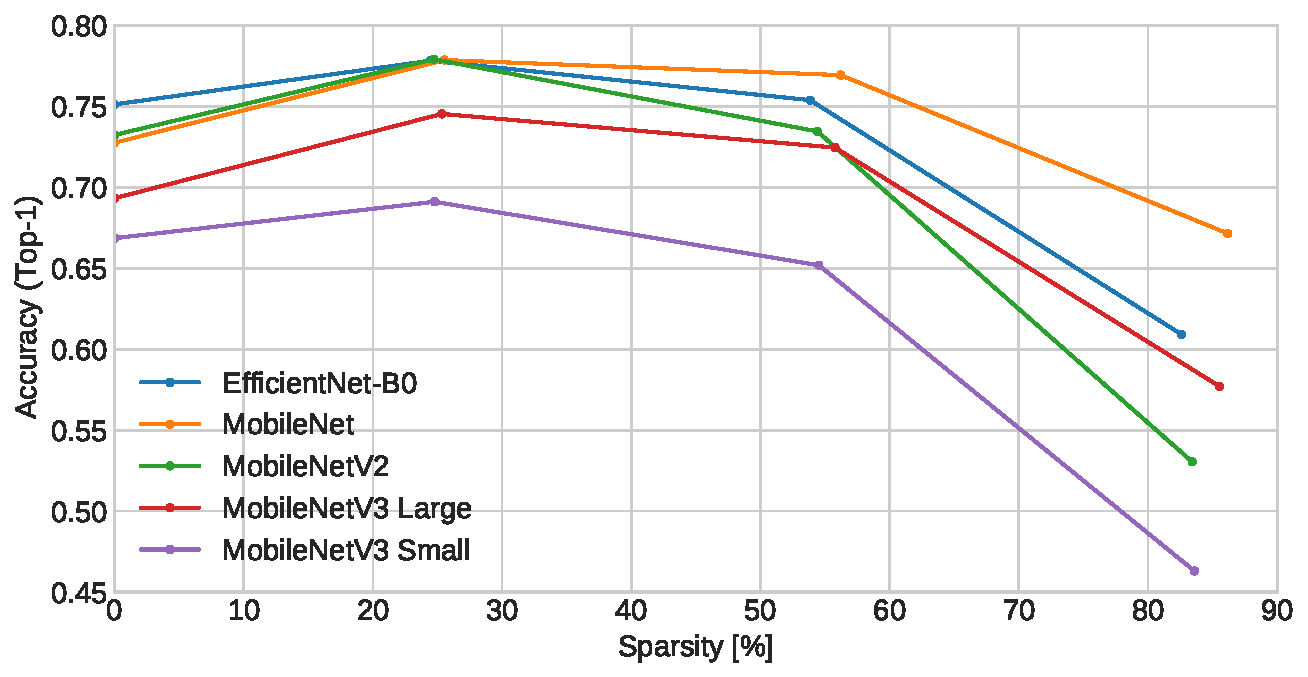
\includegraphics[width=0.7\textwidth]{img/sparsity_vs_accuracy.pdf}
\caption{Genauigkeiten (Top-1) beim Pruning auf 0\% (ungepruned), 30\%, 60\% und 90\% Sparsity}
\end{figure}

\end{frame}


\begin{frame}
\frametitle{Pruning II}

\begin{itemize}
	\item Bedarf an Hauptspeicher, Dateigröße und Inferenzzeit verändern sich durch das Pruning nicht
	\item Anwendung eines Kompressionsalgorithmus (gzip) auf die gespeicherten .tflite-Modelle
	\begin{itemize}
		\item Anwendung: z.B. Übertragung über ein Netzwerk/Internet
	\end{itemize}
\end{itemize}

\begin{figure}
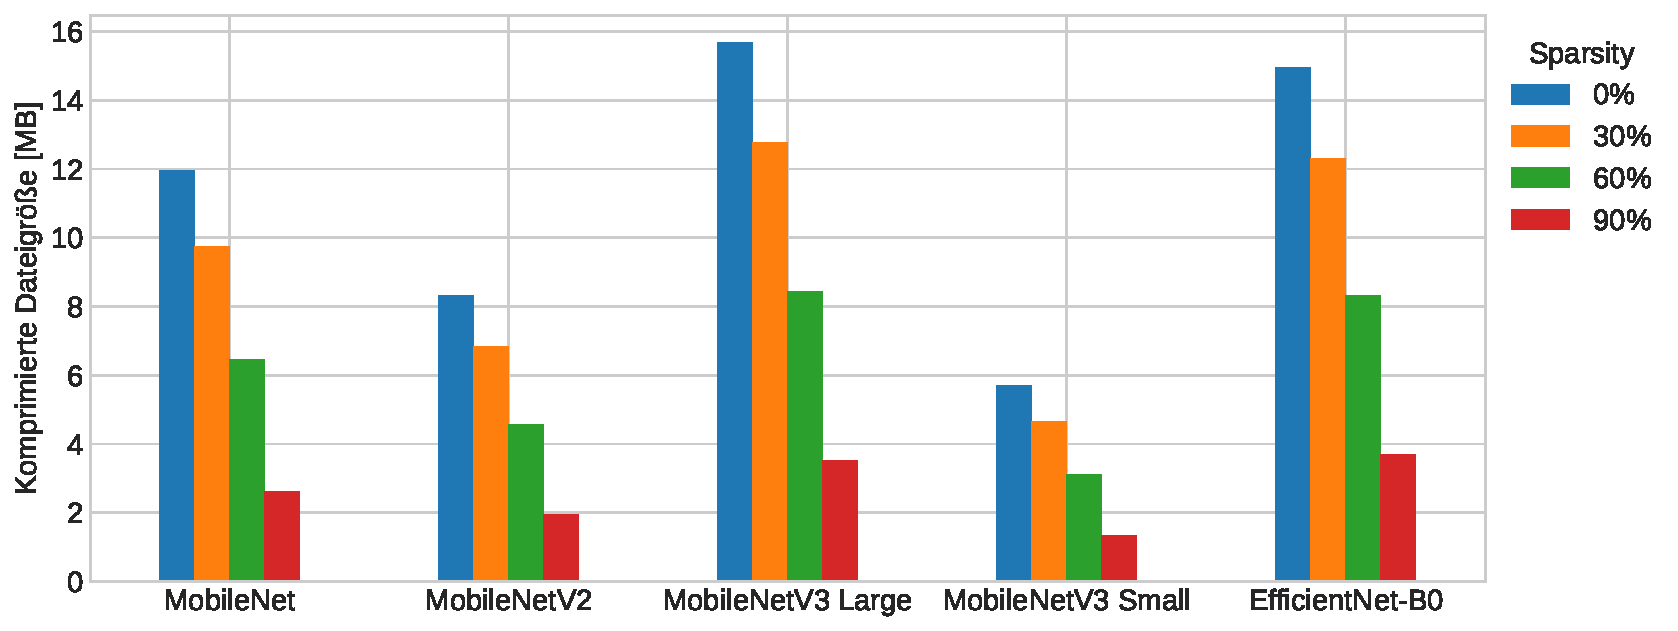
\includegraphics[width=0.8\textwidth]{img/pruned_and_compressed.pdf}
\caption{Dateigröße der Modelle nach Anwendung eines Kompressionsalgorithmus (gzip)}
\end{figure}

\end{frame}


\begin{frame}
\frametitle{Klassenweise Genauigkeit}

\begin{itemize}
	\item Ungleichmäßige Auswirkung von Pruning auf die einzelnen Klassen \cite{hooker_what_2020}
	\item Gleiches Phänomen bei der Quantisierung
\end{itemize}

\begin{figure}
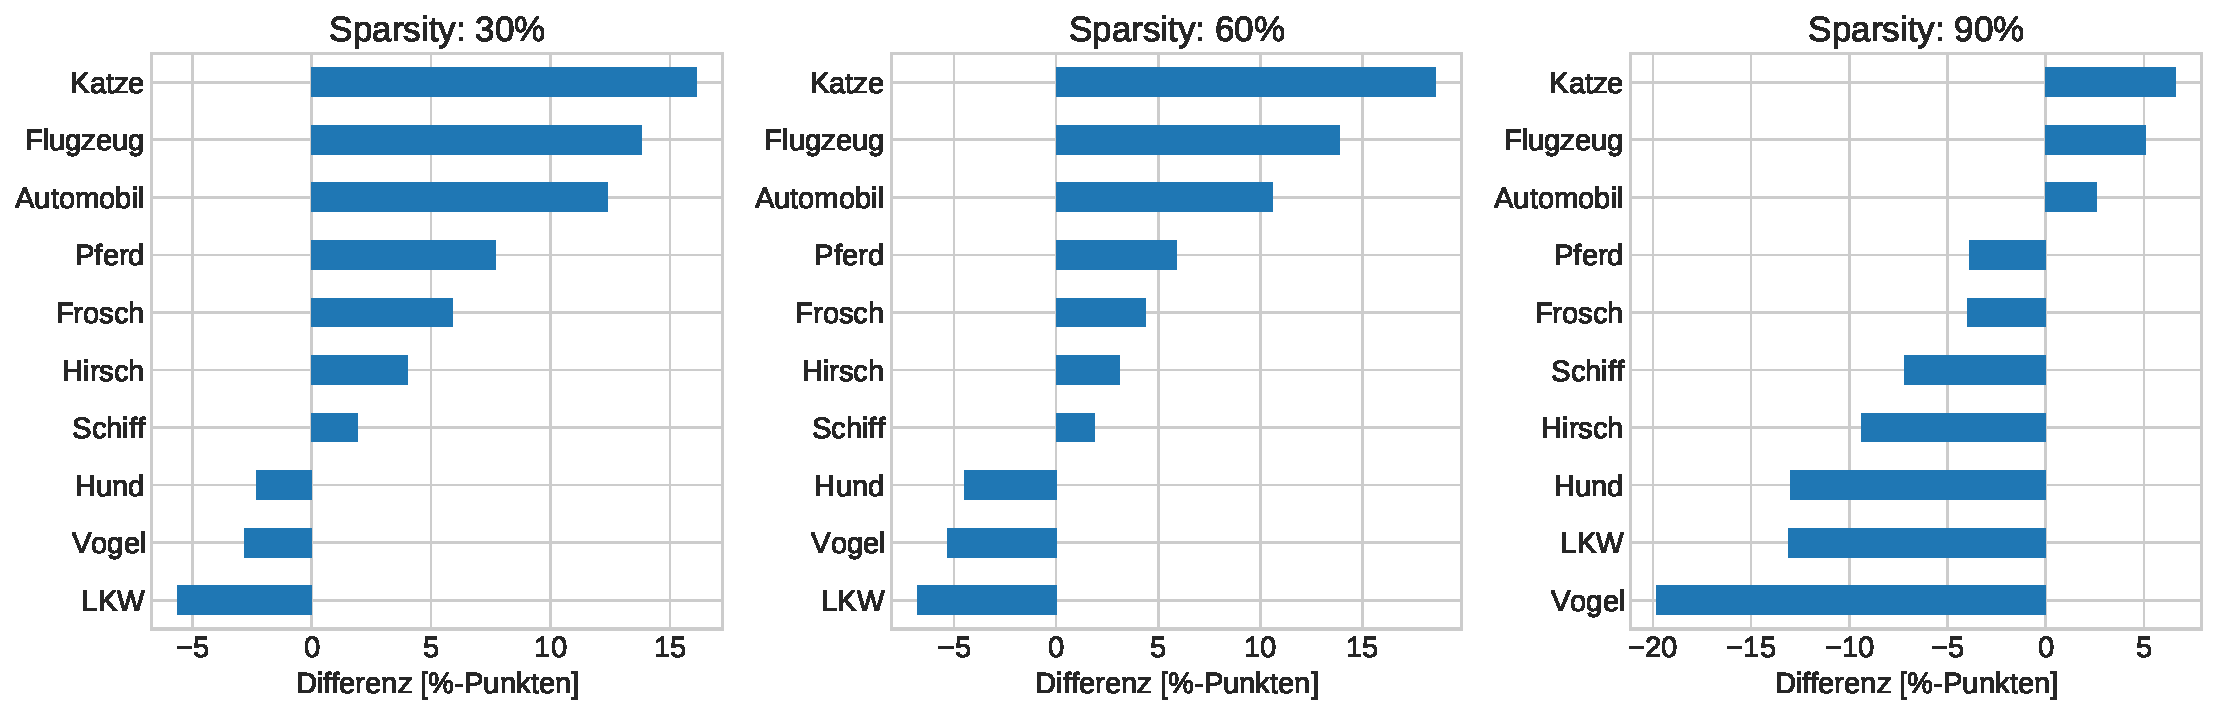
\includegraphics[width=\textwidth]{img/classwise_acc_change_pruning_mobilenet.pdf}
\caption{Veränderung der klassenweisen Top-1 Genauigkeit der geprunten MobileNet Modelle in Prozentpunkten}
\end{figure}

\end{frame}


%\section{Optimierungen}
%\begin{frame}
%\huge
%\centering
%Optimierungen
%\end{frame}


%\begin{frame}
%\frametitle{Optimierungen}
%
%\begin{itemize}
%	\item EfficientNet-lite \cite{liu_higher_2020}
%	\begin{itemize}
%		\item Squeeze-And-Excitation Module wurden entfernt
%		\item Swish Aktivierungsfunktion wurde durch ReLU6 ausgetauscht
%		\item Einige Parameter werden vom Compound Scaling ausgeschlossen
%	\end{itemize}
%	\item MobileNetV3 Minimalistic
%	\begin{itemize}
%		\item Squeeze-And-Excitation Module wurden entfernt
%		\item Hard-Swish Aktivierungsfunktion wurde durch ReLU ausgetauscht
%		\item Convolutions mit $5 \times 5$ Kernelgröße wurden durch $3 \times 3$ Kernel ausgetauscht
%	\end{itemize}
%	\item MobileNetV3 Minimalistic Modelle wurden in der Arbeit genauer betrachtet
%	\begin{itemize}
%		\item Kleinstes komprimiertes, gepruntes und quantisiertes Modell war das MobileNetV3 Small Minimalistic mit 0.36 MB Dateigröße
%	\end{itemize}
%\end{itemize}
%
%\end{frame}



%%% Abschnitt: Fazit %%%

\section{Fazit}
\begin{frame}
\huge
\centering
Fazit
\end{frame}


\begin{frame}
\frametitle{Fazit}

\begin{itemize}
	\item Quantisierung sollte in mobilen/eingebetteten Anwendungsbereichen immer in Betracht gezogen werden	
	\item Pruning ist besonders hilfreich wenn Modelle z.B. für eine Übertragung komprimiert werden sollen
	\item MobileNet Architektur verhält sich robust gegenüber Optimierungen
	\begin{itemize}
		\item Hohe Kompression mit geringen Genauigkeitsverlusten
		\item Deutlich verbesserte Inferenzzeit durch Quantisierung
		\item Durch Kombination von Pruning, Quantisierung und gzip lässt sich die Modellgröße auf 0.9 MB verringern
	\end{itemize}
	\item Klassenweise Genauigkeit sollte bei der Anwendung von Quantisierung/Pruning unbedingt beachtet werden
\end{itemize}

\end{frame}



%%% Abschnitt: Literaturverzeichnis %%%

\section{Literaturverzeichnis}
\begin{frame}
\huge
\centering
Literaturverzeichnis
\end{frame}


\begin{frame}[allowframebreaks]
\frametitle{Literaturverzeichnis}
\bibliographystyle{alpha}
\bibliography{references/references.bib}
\end{frame}

\end{document}
